\mychapter{Credential Relationship Binding Nullifier}
Anonymous credential systems enable users to prove statements about their identity while maintaining privacy. In Chapters 2 and 3, we advanced from single-issuer Attribute-Based Anonymous Credentials ($\ABC$) to a Multi-Issuer Multi-Credential system ($\MIMCABC$) that securely binds credentials from different issuers to the same identity. However, practical identity frameworks require two additional capabilities: hierarchical credential organization and sybil resistance.

Real-world credentials naturally form a hierarchy, this is notable when applying for bank loans or new credentials from the government that require multiple credentials shown together, a naive request without privacy but challenging to implement in a privacy-preserving identity system. Consider a user with both a passport and a driver's license, as shown in Figure~\ref{fig:credential-nullifier}, the passport functions as a foundational Master Credential containing a secret key $\k$, while the driver's license is a Context Credential tied to a specific domain $\ctx$. For privacy and security, we need to cryptographically bind these credentials together and prevent users from obtaining multiple credentials for the same context (e.g., multiple driver's licenses) without compromising anonymity.

\begin{figure}
        \begin{pchstack}[boxed, center, space=4em]
            \begin{pcvstack}
                \procedure[space=auto]{Master Credential (Passport)}{%
                \id: 12345, \\
                \ctx: "master", \\
                \exp: "10/11/2026", \\
                \k: 54321
                }
            \end{pcvstack}
            \pcvspace
            \begin{pcvstack}
                \procedure[space=auto]{Context Credential (Driver's License)}{%
                 \id: 12345, \\
                 \ctx: "DMV", \\
                 \exp: "10/11/2028"
                }
            \end{pcvstack}
        \end{pchstack}
        \begin{center}
        \begin{tikzpicture}
            \draw[->, thick] (-2,0) -- (-1,-1);
            \draw[->, thick] (2,0) -- (1,-1);
        \end{tikzpicture}
        \end{center}
        \begin{pchstack}[boxed, center]
            \begin{pcvstack}
                \procedure[space=auto]{Nullifier}{%
                 \textsf{n} = 1/(\k + \text{"DMV"}) \\
                 \nul = g^{\textsf{n}} 
                }
            \end{pcvstack}
        \end{pchstack}
    \caption{A credential hierarchy with a nullifier that binds a context credential to a master credential. The nullifier combines the master credential's secret key $\k$ with the context identifier "DMV" through a one-way function, creating a unique, verifiable binding that prevents sybil attacks while maintaining privacy.}
    \label{fig:credential-nullifier}
\end{figure}

This presents a core technical challenge: \emph{How can we create a nullifier that cryptographically proves the relationship between two separate credentials without revealing the underlying attributes or enabling tracking across verifications?}

\section{SHOULD WE INCLUDE A CHAPTER ROADMAP?}

% \subsection*{Chapter Organization}
% The remainder of this chapter is organized as follows: Section 4.3 introduces our pairing-free VRF construction in prime-order groups. Section 4.4 presents our zero-knowledge proof protocol for multiplicative inverse relationships. Section 4.5 combines these components to construct the complete Credential Relationship Binding Nullifier (CRBN) system and demonstrates its integration with our identity framework. Finally, Section 4.6 provides a comprehensive performance evaluation comparing our approach to existing techniques.


\subsection{Technical Challenges and Approach}

Creating an efficient, privacy-preserving nullifier for credential binding raises three specific challenges:
\begin{enumerate}
    \item \textbf{Efficient Verification}: The nullifier must be verifiable without expensive bilinear pairings while maintaining provable uniqueness and verifiable pseudorandomness.
    
    \item \textbf{Privacy Preservation}: Verification must not reveal the master credential's key $\k$ or the context credential's identifier $\ctx$, nor enable credential linking.
    
    \item \textbf{Integration with $\MIMCABC$}: The nullifier mechanism must seamlessly extend our existing anonymous credential framework without compromising its security properties.
\end{enumerate}

Our approach leverages and extends Verifiable Random Functions (VRFs) to address these challenges. Specifically, we:

\begin{enumerate}
    \item Start with the Dodis-Yampolskiy VRF~\cite{hutchison_verifiable_2005}, which computes $y = e(g, \tilde{g})^{1/(sk+x)}$ in bilinear groups
    
    \item Develop a pairing-free variant that operates entirely in prime-order groups
    
    \item Create novel $\Sigma$-protocols for proving relationships between committed attributes and nullifiers and of independent interest
    
    \item Design a complete credential binding system that prevents sybil attacks while maintaining privacy
\end{enumerate}

\subsection{Related Work}

\begin{table}
\begin{center}
\caption{Comparison of Nullifier/VRF Schemes for Credential Binding}
\label{tab:nullifier-comparison}
\begin{tabular}{l|cccccc}
\toprule
\textbf{Scheme} & 
\textbf{Pairing-} & 
\textbf{Private} & 
\textbf{Unlinkable}  & 
\textbf{Deterministic} & 
\textbf{Proof} & 
\textbf{Relative} \\
 & 
 \textbf{Free} & 
 \textbf{Inputs}$^1$ & 
 \textbf{Outputs}$^2$ & 
 \textbf{Value}$^3$ & 
 \textbf{Type} & 
 \textbf{Ver. Time}$^4$ \\
\midrule
DY VRF \cite{hutchison_verifiable_2005} & \ding{55} & \ding{55} & \ding{55} & \ding{51} & Pairing & 3x slower \\
CanDID \cite{maram2021candid} & \ding{51} & \ding{51} & \ding{55} & \ding{51} & MPC & Very slow \\
TACT/S3ID \cite{rabaninejad_attribute-based_2024} & \ding{55} & \ding{51} & \ding{55} & \ding{51} & Groth Sahai + Pairing & ~1.5-2x slower \\
SyRA \cite{crites_syra_2024} & \ding{55} & \ding{51} & \ding{55} & \ding{51} & Sigma+Pairing & ~1.5-2x slower \\
UTT Nullifier \cite{tomescu2022utt} & \ding{55} & \ding{51} & \ding{51} & \ding{51} & Sigma+Pairing & 1.5x slower \\
\textbf{Our CRBN} & \ding{51} & \ding{51} & \ding{51} & \ding{51} & Sigma only & 1x (baseline) \\
\bottomrule
\end{tabular}
\end{center}
\vspace{1em}
\footnotesize{$^1$Operates on inputs (e.g., secret keys, attributes) hidden in commitments.} \\
\footnotesize{$^2$Nullifier can be presented as a commitment for unlinkability.} \\
\footnotesize{$^3$Ensures a unique underlying nullifier value per user-context pair for sybil resistance.} \\
\footnotesize{$^4$Approximate verification time relative to CRBN, based on benchmarks in Section X.}
\end{table}

Previous systems have addressed aspects of hierarchical credential binding and sybil resistance, but all have significant limitations:

\begin{itemize}
    \item \textbf{UTT}~\cite{tomescu2022utt} uses a similar approach to ours for anonymous payments, creating serial numbers (nullifiers) from a registration credential. However, UTT relies on bilinear pairings, introducing substantial computational overhead.
    
    \item \textbf{CanDID}~\cite{maram2021candid} clearly defines the master/context credential relationship but compromises privacy by maintaining mappings between credential public keys, enabling linkability across interactions.
    
    \item \textbf{Pairing-based systems} like SyRA~\cite{crites_syra_2024} and S3ID~\cite{rabaninejad_attribute-based_2024} implement hierarchical credentials but suffer from efficiency issues due to their reliance on pairings and S3ID uses Groth Sahai proofs which are less efficient than $\Sigma$-protocols.
    
    \item \textbf{Standard VRFs}~\cite{hutchison_verifiable_2005} could generate unique nullifiers but use pairings and reveal the user's public key during verification, compromising anonymity.
\end{itemize}

While our $\MIMCABC$ system (Chapter 3) provides efficient identity binding across multiple credentials, it doesn't address the hierarchical relationship between credentials or prevent a user from obtaining multiple credentials for the same context. This chapter fills that gap.

\subsection{Contributions}

We advance anonymous credential systems with three key contributions:

\begin{enumerate}
    \item \textbf{Pairing-Free VRF Construction}: We redesign the Dodis-Yampolskiy VRF for standard prime-order groups, eliminating pairings while maintaining security under the $q$-DDHI assumption. Our construction transforms $y = e(g, \tilde{g})^{1/(sk+x)}$ to $y = g^{1/(sk+x)}$ with a novel verification approach. We show a 3.1x speedup of our construction against the DY VRF. 
    
    \item \textbf{Zero-Knowledge Protocols for Inverse Relations}: We develop efficient $\Sigma$-protocols to prove knowledge of committed inverse exponents—a crucial building block for private nullifier verification. These protocols enable statements of the form:
    \[
    \zkpok\{(sk, x, r_1, r_2) : \cm_1 = g_1^{sk}g^{r_1} \land \cm_2 = g_2^{x}g^{r_2} \land y = g^{1/(sk+x)}\}
    \]
    
    \item \textbf{Credential Relationship Binding Nullifier (CRBN)}: We integrate these components into a complete system that binds master credentials to context credentials via nullifiers. Our two constructions, 1) producing a deterministic nullifier and 2) producing a committed nullifier, are respectively 5.5x and 2.9x faster for  $\VRFEval+\VRFProve$ and 4.6x and 3.9x faster for $\VRFVerify$ compared to the fastest pairing-based alternative we found \cite{tomescu2022utt}.
\end{enumerate}

These contributions enable a privacy-preserving credential hierarchy with sybil resistance, addressing a critical gap in existing anonymous credential systems. Our approach maintains the privacy guarantees of $\MIMCABC$ while adding the ability to enforce context-specific uniqueness—balancing privacy with the accountability requirements of real-world identity systems.






\section{Preliminaries}

\subsection{Cryptographic Assumptions}

\begin{definition}[q-DDHI Assumption]
Let $\mathbb{G}$ be a cyclic group of prime order $p$ with generator $g$. The $q$-Decisional-Diffie-Hellman Inversion ($q$-DDHI) \cite{mitsunari_new_2002} assumption states that for any PPT adversary $\mathcal{A}$, there exists a negligible function $\negl$ such that:
\[
\left|\Pr\left[ x \sample \Zp^*, b \sample \{0,1\}, z_0 = g^{1/x}, z_1 \sample \G : \mathcal{A}(g, g^x, g^{x^2}, \ldots, g^{x^q}, z_b) = b \right] - \frac{1}{2}\right| \leq \negl(\lambda)
\]
Informally, given $(g, g^x, g^{x^2}, \ldots, g^{x^q})$, no PPT adversary can distinguish $g^{1/x}$ from a random group element with non-negligible advantage.
\end{definition}

\begin{remark}
The $q$-DDHI assumption is a variant of the $(q+1)$-generalized Diffie-Hellman assumption as shown by Boneh and Boyen \cite{kanade_efficient_2004}. This assumption directly underpins the security of our pairing-free VRF construction.
\end{remark}

\begin{definition}[$q$-DBDHI Assumption]
Let $\mathbb{G}_1, \mathbb{G}_2, \mathbb{G}_T$ be cyclic groups of prime order $p$ with a bilinear pairing $e: \mathbb{G}_1 \times \mathbb{G}_2 \to \mathbb{G}_T$, and generators $g \in \mathbb{G}_1$, $\tilde{g} \in \mathbb{G}_2$. The $q$-Decisional-Bilinear Diffie-Hellman Inversion ($q$-DBDHI) assumption states that for any PPT adversary $\mathcal{A}$, there exists a negligible function $\negl$ such that:
\[
\left| \Pr\left[ x \sample \Z_p^*, b \sample \{0,1\}, z_0 = e(g, \tilde{g})^{1/x}, z_1 \sample \G_T : \mathcal{A}(g, g^x, g^{x^2}, \ldots, g^{x^q}, \tilde{g}, z_b) = b \right] - \frac{1}{2}\right| \leq \negl(\lambda)
\]
Informally, no PPT adversary can distinguish $e(g, \tilde{g})^{1/x}$ from a random element in $\mathbb{G}_T$ given $(g, g^x, \ldots, g^{x^q}, \tilde{g})$ with non-negligible advantage.
\end{definition}


\subsection{Building Blocks}

\subsubsection{Pedersen Vector Commitments}
We use position-binding Pedersen Commitments from Chapter 2, which allow committing to a vector of messages while hiding the values. For a message vector $[\id, \ctx, \exp, \k]$ and randomness $\usk$, the commitment is:
\[
\cm = \CMCom([m_1, \ldots, m_n];\usk) = g_1^{m_1} \cdots g_n^{m_n} g^\usk
\]

Pedersen Commitments provide three key properties:
\begin{itemize}
    \item \textbf{Hiding}: The commitment reveals no information about the committed values.
    \item \textbf{Binding}: It's computationally infeasible to open a commitment to different values.
    \item \textbf{Position-Binding}: Each position in the vector is cryptographically bound to its specific base element, preventing attribute swapping.
\end{itemize}


\subsubsection{Verifiable Random Functions}
A Verifiable Random Function (VRF) \cite{micali_verifiable_1999, hutchison_verifiable_2005} is a pseudorandom function that provides proofs of correct evaluation. Following \cite{bitansky_verifiable_2020}, a VRF consists of these algorithms:

\begin{definition}[Verifiable Random Function]
A VRF is a tuple of PPT algorithms \\
$(\VRFGen, \VRFEval, \VRFProve, \VRFVerify)$ with message space $\mathcal{X}$, output space $\mathcal{Y}$ and proof space $\Pi$ where:
\begin{itemize}
    \item $\VRFGen(1^\lambda) \to (sk, pk)$: Generates a secret key $sk$ and public key $pk$.
    \item $\VRFEval(sk,x) \to y$: Computes the VRF output $y \in \mathcal{Y}$ for input $x \in \mathcal{X}$ using secret key $sk$.
    \item $\VRFProve(sk,x) \to \pi$: Produces a proof $\pi \in \Pi$ that $y = \VRFEval(sk,x)$ is computed correctly.
    \item $\VRFVerify(pk,x,y,\pi) \to \{0,1\}$: Verifies that $y$ is the correct VRF output for input $x$ using proof $\pi$.
\end{itemize}
\end{definition}

A secure VRF must satisfy the following properties:

\begin{itemize}
    \item \textbf{Completeness:} Honest evaluation and proof generation always passes verification:
    \[
    \Pr\left[ \VRFVerify(pk,x,y,\pi) = 1 \ \middle| \ 
    \begin{array}{l}
        (sk, pk) \leftarrow \VRFGen(1^\lambda) \\
        y = \VRFEval(sk,x) \\
        \pi \leftarrow \VRFProve(sk,x)
    \end{array}
    \right] = 1
    \]
    
    \item \textbf{Uniqueness:} For each input $x$ and public key $pk$, only one output $y$ can be verified:
    \[
    \text{if} \quad \VRFVerify(pk, x, y_0, \pi_0) = \VRFVerify(pk, x, y_1, \pi_1) = 1 \quad \text{then} \quad y_0 = y_1
    \]
    
    \item \textbf{Pseudorandomness:} The VRF output is indistinguishable from random for any input not previously queried, defined by the following game $\mathcal{G}_{\mathcal{A}}^{\text{vrf}}$:
    \begin{enumerate}
        \item The VRF challenger samples $(sk, pk) \leftarrow \VRFGen(1^\lambda)$, and sends $pk$ to $\mathcal{A}$.
        \item $\mathcal{A}$ submits evaluation queries $x_1, \ldots, x_Q \in \mathcal{X}$, and receives $(y_i, \pi_i)$ for each query, where $y_i = \VRFEval(sk, x_i)$ and $\pi_i \leftarrow \VRFProve(sk, x_i)$.
        \item At any point, $\mathcal{A}$ submits a challenge input $x_* \in \mathcal{X}$ such that $x_* \not\in \{x_1, \ldots, x_Q\}$.
        \item The challenger computes $y_0^* = \VRFEval(sk, x_*)$, samples $y_1^* \sample \mathcal{Y}$ uniformly at random, then samples $b \sample \{0,1\}$ and sends $y_b^*$ to $\mathcal{A}$.
        \item $\mathcal{A}$ may continue to make evaluation queries for inputs other than $x_*$.
        \item At the end, $\mathcal{A}$ outputs a guess $b'$. The game outputs 1 if $b' = b$, and 0 otherwise.
    \end{enumerate}
    
    We say that the VRF satisfies pseudorandomness if for all PPT adversaries $\mathcal{A}$:
    \[
    \text{Adv}_{\mathcal{A}}^{\text{vrf}} := \left|\Pr\left[\mathcal{G}_{\mathcal{A}}^{\text{vrf}}(\lambda) = 1\right] - \frac{1}{2}\right| \leq \text{negl}(\lambda)
    \]
\end{itemize}


    
In our work, we focus on adapting the Dodis-Yampolskiy VRF \cite{hutchison_verifiable_2005}, which computes $y = e(g, \tilde{g})^{1/(sk+x)}$ in bilinear groups, to work efficiently in standard prime-order groups without pairings.

\subsubsection{Zero-Knowledge Proofs and Sigma-Protocols}
Our credential binding mechanism relies on zero-knowledge proofs, particularly Sigma-protocols, to verify relations between committed values without revealing them.

A Sigma-protocol is a three-move interactive proof system where:
\begin{enumerate}
    \item The prover $\mathcal{P}$ sends a commitment message $a$.
    \item The verifier $\mathcal{V}$ sends a random challenge $e$.
    \item The prover responds with $z$, and $\mathcal{V}$ accepts if the verification equation holds.
\end{enumerate}
These protocols satisfy:
\begin{itemize}
    \item \textbf{Completeness}: For all $(x,w) \in \mathcal{R}$, an honest prover always convinces the verifier.
    \item \textbf{Special Soundness}: There exists an efficient extractor $\mathcal{E}$ such that, given any statement $x$ and two accepting transcripts $(a,e,z)$ and $(a,e',z')$ with $e \neq e'$, $\mathcal{E}$ can extract a witness $w$ such that $(x,w) \in \mathcal{R}$.
    \item \textbf{Special Honest-Verifier Zero-Knowledge}: There exists an efficient simulator $\mathcal{S}$ that, given a statement $x$ and a challenge $e$, produces a transcript $(a,e,z)$ that is computationally indistinguishable from a real transcript between an honest prover and verifier, without using a witness.
\end{itemize}



\section{Technical Overview and Approach}\label{sec:overview}

The three core challenges we solve are: 1) remove pairings from DY's VRF, 2) preserve privacy, and 3) enable unlinkability. This section provides a roadmap of our approach before we detail each construction.

\begin{figure}[ht]
\centering
\begin{tikzpicture}[
    node distance=1.5cm,
    box/.style={rectangle, rounded corners, draw, fill=white, text width=2.5cm, minimum height=1.2cm, align=center, font=\small},
    arrow/.style={thick,->,>=stealth},
    improvement/.style={text width=2.2cm, align=center, font=\footnotesize\itshape}
]
% Nodes
\node[box] (dy) {
    \textbf{Dodis-Yampolskiy VRF}
};

\node[box, right=of dy] (dypf) {
    \textbf{Ch 1. Pairing-Free VRF (DY-PF)}
};

\node[box, right=of dypf] (private) {
    \textbf{Ch 2. Privacy-Preserving VRF}
};

\node[box, right=of private] (crbn) {
    \textbf{Ch 3. Privacy-Preserving Unlinkable VRF}
};

% Arrows 
\draw[arrow] (dy.east) -- (dypf.west);
\draw[arrow] (dypf.east) -- (private.west);
\draw[arrow] (private.east) -- (crbn.west);

% Improvement text below arrows
\node[improvement, below=1cm of dy.east] (imp1) {Eliminates pairings for 3.1× performance gain};
\node[improvement, below=1cm of dypf.east] (imp2) {Enables operations on hidden attributes};
\node[improvement, below=1cm of private.east] (imp3) {Adds unlinkability while maintaining verifiability};

\end{tikzpicture}
\caption{Overview of our construction approach, progressing from the original Dodis-Yampolskiy VRF to our final Credential Relationship Binding Nullifier (CRBN).}
\label{fig:vrf-construction-overview}
\end{figure}

To understand our contributions, we examine the core technical challenges in creating an efficient, privacy-preserving nullifier mechanism for hierarchical credential systems. Consider a user with a master credential (containing secret key $\k$, denoted as $sk$ below) who needs to prove possession of a context credential (with identifier $\ctx = \text{"DMV"}$, denoted as $x$) without revealing their identity or allowing them to obtain multiple DMV credentials.


\subsection{Challenge 1: Creating a Pairing-Free Nullifier}

The Dodis-Yampolskiy \cite{hutchison_verifiable_2005} VRF provides an elegant solution for generating unique, pseudorandom nullifiers using $y = e(g, \tilde{g})^{1/(sk+x)}$ in bilinear groups. We wish to improve on the efficiency and privacy. 

\subsubsection{Can we remove Bilinear Pairings from DY VRF?}

We start with the challenge of removing pairings from the DY VRF. DY VRF achieves verifiability:

\begin{itemize}
    \item The verifier confirms $\pi = \tilde{g}^{1/(sk+x)}$ is valid via $e(g^x \cdot pk, \pi) = e(g^{sk+x}, \tilde{g}^{1/(sk+x)}) = e(g, \tilde{g})$
    \item Then checks $y = e(g, \pi) = e(g, \tilde{g})^{1/(sk+x)}$
\end{itemize}

Verification depends on the bilinearity property $e(g^a, \tilde{g}^b)^c = e(g, \tilde{g})^{abc}$, which enables "exponent multiplication" across groups, allowing the transformations
\[
e(g^x \cdot pk, \pi) \quad \stackrel{?}{=} \quad e(g^{sk+x}, \tilde{g}^{1/(sk+x)}) \quad \stackrel{?}{=} \quad 
 e(g, \tilde{g})^{(sk+x)/(sk+x)} \quad  \stackrel{}{=} \quad e(g, \tilde{g})
\]
\[
y \quad \stackrel{?}{=} \quad e(g, \pi) \quad \stackrel{?}{=} \quad e(g,\tilde{g}^{1/(sk+x)}) \quad \stackrel{}{=} \quad e(g, \tilde{g})^{1/(sk+x)}
\]

Security relies on the $q$-DBDHI problem which states that given $(g, g^x, g^{x^2}, \ldots, g^{x^q}, \tilde{g})$, no $\PPT$ adversary can distinguish between $e(g,\tilde{g})^{1/x}$ and a uniform element in $\G_T$ with non-negligible advantage , ensuring the VRF outputs maintain pseudorandomness after the adversary has observed $(x',y',\pi')$ pairs.

\subsubsection{The Prime-Order Group Challenge}

Prime-order groups without pairings don't have the bilinearity property, given $pk = g^{sk}$, $x$, and $y = g^{1/(sk+x)}$, standard group operations cannot directly verify the relationship. For example, given $pk  \cdot g^x = g^{sk+x}$, attempts fail to equate or cancel out:

\begin{enumerate}
    \item $g^{sk+x} \cdot g^{1/(sk+x)} = g^{sk+x+1/(sk+x)}$
    \item $g^{sk+x}/g^{1/(sk+x)} = g^{(sk+x)^2-1/(sk+x)}$
\end{enumerate}

Our insight is to reverse the verification approach. Instead of trying to derive $g^{1/(sk+x)}$ from $g^{sk+x}$ or cancel with a reciprocal, we use a zero knowledge proof $\Sigma$-protocol to verify that $y$ raised to the power $(sk+x)$ equals $g$. In doing so, our pairing-free construction shifts from the $q$-DBDHI assumption to the $q$-DDHI assumption. This gives us the relation:

\[
\mathcal{R}_{\mathsf{DY-PF}} = \left\{ 
\begin{array}{l} 
(\pk, x, y),\\
(sk) 
\end{array}
\ \middle|
\ \begin{array}{l}
pk = g^{sk} \\
y^{sk + x} = g  \\
\end{array} \right\}
\]

\subsection{Challenge 2: Privacy-Preserving Credential Binding}

Even with a pairing-free solution, standard VRFs reveal the public key $pk = g^{sk}$ and the input $x$,  compromising credential anonymity. In our hierarchical credential system, $sk$ and $x$ are committed attributes in different credentials that must remain private. We solve this through a two-step approach: first, addressing the simpler case of a single committed exponent, then extending to linear combinations.

\subsubsection*{Step 1. Proving Knowledge of a Committed Inverse}
Our first insight is reducing this problem to the problem of proving knowledge of a (committed) inverse exponent which is congruent to proving a DDHI challenge $g^{1/x}$
\[
\mathcal{R}_{\mathsf{DDHI}} = \left\{ 
\begin{array}{l} (\cm, y),\\
(x, r) 
\end{array}
\ \middle|
\ \begin{array}{l}
\cm = g_1^{x} g^r \\
y = g^{1/x} \\
\end{array} \right\}
\]

We use a $\Sigma$-protocol to prove knowledge of the exponents $x, r$; during the protocol, we use the same random coin and response from $x$ to show the relation $y^x (=g)$ holds, and therefore $y$ must commit to $x$. We show the full protocol \ref{pok-committed-inverse-exponent}. 

\subsubsection*{Step 2. Proving Knowledge of a Committed Inverse Linear Relation}

We then extend this to prove a linear relation of inverse exponents $y = g^{1/(sk+x)}$ where $sk$ and $x$ come from different commitments, enforcing a relation $\mathcal{R}_{\mathsf{nullifier}}$ holds. We show the full protocol here \ref{pok-committed-inverse-linear-relation}. 

\[
\mathcal{R}_{\mathsf{nullifier}} = \left\{ 
\begin{array}{l} (\cm_1, \cm_2, y),\\
(sk, x, r_1, r_2) 
\end{array}
\ \middle|
\ \begin{array}{l}
\cm_1 = g_1^{sk} g^{r_1} \\
\cm_2 = g_2^{x} g^{r_2} \\
y = g^{1/(sk + x)} \\
\end{array} \right\}
\]


\subsection{Challenge 3: Unlinkable Credential Presentations}

A deterministic nullifier $y = g^{1/(sk+x)}$ is necessary for Sybil resistance ensuring a unique, verifiable value for each $(sk,x)$ pair. However, deterministic algorithms create privacy problems with linkability. There are many use-cases for the verifiable connection of $(sk, x)$, such as revocation accumulators, which a user would need to interact with frequently, requiring a probabilistic output that can verify the $(sk+x)$ connection. 

Our solution is to commit to the nullifier rather than revealing it directly:
\[
\cm_{\mathsf{null}} = g_3^{1/(sk+x)} g^{r_3}
\]

We must now prove that the committed value represents the nullifiers $(sk+x)$, we do so with the following relation:


\[
\mathcal{R}_{\mathsf{CommittedNull}} = \left\{ 
\begin{array}{l} 
(\cm_1, \cm_2, \cm_3, \cm_4), \\
(sk, x, r_1, r_2, r_3, r_4) 
\end{array}
\ \middle| \
\begin{array}{l}
\cm_1 = g_1^{sk} g^{r_1} \\
\cm_2 = g_2^{x} g^{r_2} \\
\cm_3 = g_3^{1/(sk + x)} g^{r_3}  \quad \text{\small{The Committed Nullifier}}\\
\cm_4 = \cm_3^{sk + x} g^{r_4} = g_3 g^{r_3 (sk + x) + r_4}
\end{array} \right\}
\]

The auxiliary commitment $\cm_4$ enables verification analogous to our approach in Challenge 1: instead of verifying $y^{sk+x} = g$ directly, we prove that $\cm_3^{sk+x} = g_3$ (modulo some randomness $g^{r_4}$). This algebraic relationship can only hold if $\cm_3$ commits to $g_3^{1/(sk+x)}$, thus verifying the correctness of the committed nullifier without revealing it.

This construction extends our technique from Challenge 2 by applying the exponentiation-inversion verification paradigm entirely within the commitment space. The verification operates on the same mathematical principle ($x \cdot \frac{1}{x} = 1$), but now uses homomorphic properties of Pedersen commitments to prove the relationship between committed values, enabling both unlinkable presentations and verifiable credential binding.




\subsection{Our Approach}

To address these challenges, we develop a series of progressively more sophisticated cryptographic constructions:

\begin{enumerate}
    \item \textbf{Pairing-Free VRF (DY-PF):} We design a $\Sigma$-protocol that enables verification of $y = g^{1/(sk+x)}$ without pairings by proving the relation $y^{sk+x} = g$, preserving the security properties of the original DY VRF but with significantly improved efficiency.
    
    \item \textbf{Privacy-Preserving VRF:} We extend our technique to verify nullifiers computed from committed attributes, creating novel $\Sigma$-protocols for proving inverse exponent relations between commitments.
    
    \item \textbf{Committed Nullifier:} We further develop our framework to commit the nullifier itself, enabling unlinkable credential presentations while maintaining Sybil resistance.
\end{enumerate}

Each construction builds upon the previous one, culminating in the Credential Relationship Binding Nullifier (CRBN) that satisfies all our requirements for hierarchical, privacy-preserving, and efficient credential systems.









\section{Pairing-Free VRF Construction}\label{sec:pairing-free-vrf}
In this section, we develop our pairing-free VRF (DY-PF), but first, we review the original DY VRF.

The Dodis-Yampolskiy VRF~\cite{hutchison_verifiable_2005} operates in a bilinear group setting with prime-order groups $\mathbb{G}_1$, $\mathbb{G}_2$, and $\mathbb{G}_T$, with a Type-3 pairing $e: \mathbb{G}_1 \times \mathbb{G}_2 \rightarrow \mathbb{G}_T$. Let $g \in \mathbb{G}_1$ and $\tilde{g} \in \mathbb{G}_2$ be generators. The construction is as follows:

\begin{itemize}
    \item $\mathsf{VRF.Gen}(1^\lambda) \to (sk, pk)$: Sample $sk \sample \mathbb{Z}_p^*$, compute $pk = g^{sk} \in \mathbb{G}_1$. Output $(sk, pk)$.
    
    \item $\mathsf{VRF.Eval}(sk, x) \to y$: Compute $y = e(g, \tilde{g})^{1/(sk + x)} \in \mathbb{G}_T$.
    
    \item $\mathsf{VRF.Prove}(sk, x) \to \pi$: Compute proof $\pi = \tilde{g}^{1/(sk + x)} \in \mathbb{G}_2$.
    
    \item $\mathsf{VRF.Vfy}(pk, x, y, \pi) \to \{0, 1\}$: Verify two equations:
    \begin{align}
        e(g^{x} \cdot pk, \pi) &\stackrel{?}{=} e(g, \tilde{g}) \quad \text{(Equation 1)}\\
        y &\stackrel{?}{=} e(g, \pi) \quad \text{(Equation 2)}
    \end{align}
\end{itemize}

The security of this VRF rests upon the $q$-Decisional Bilinear Diffie-Hellman Inversion ($q$-DBDHI) assumption, which states that given $(g, g^{sk}, g^{(sk)^2}, \ldots, g^{(sk)^q})$ and $\tilde{g}$, the value $e(g, \tilde{g})^{1/(sk+x)}$ is computationally indistinguishable from a random element in $\mathbb{G}_T$.

The pairing-based verification provides information-theoretic uniqueness, but at the cost of the pairing. Our goal is to preserve the security properties while eliminating pairings.

\subsection{Pairing-Free Construction (DY-PF)}\label{sec-dy-pf}

Our VRF operates in a prime-order group $\mathbb{G}$ of order $p$ with generator $g$. The message space is $\mathcal{X} = \mathbb{Z}_p$, the output space is $\mathcal{Y} = \mathbb{G}$, and the proof space is $\Pi = \mathbb{G} \times \mathbb{G} \times \mathbb{Z}_p$.

\subsection{Construction}

Our VRF operates in a prime-order group $\mathbb{G}$ of order $p$ with generator $g$. The message space is $\mathcal{X} = \mathbb{Z}_p$, the output space is $\mathcal{Y} = \mathbb{G}$, and the proof space is $\Pi = \mathbb{G} \times \mathbb{G} \times \mathbb{Z}_p$. The algorithms are defined as follows:

\begin{itemize}
    \item $\mathsf{VRF.Gen}(1^\lambda) \to (sk, pk)$: Sample $sk \sample \mathbb{Z}_p^*$, compute $pk = g^{sk}$, and output $(sk, pk)$.
    \item $\mathsf{VRF.Eval}(sk, x) \to y$: Compute $y = g^{1/(sk + x)} \in \mathbb{G}$.
    \item $\mathsf{VRF.Prove}(sk, x) \to \pi$: Generate proof $\pi$ using the $\Sigma$-protocol described below.
    \item $\mathsf{VRF.Verify}(pk, x, y, \pi) \to \{0, 1\}$: Output 1 if $\pi$ verifies $y$ correctly per the $\Sigma$-protocol, else 0.
\end{itemize}

\begin{remark}
    Verifying $\VRFVerify(pk, x, \VRFEval(sk, x) \to y) \to 1$ is a naive verification approach without a proof which yeilds a Verifiable Unpredictable Function (VUF), not a VRF because it lacks the mechanism to prove pseudorandomness to a verifier. DY uses pairings to bridge the gap, we replace pairings with a $\Sigma$-protocol. 
\end{remark}

\subsection{Proof Protocol}
\begin{protocol}{P-DY Proof Protocol}{}\label{protocol-pdy-protocol1}
\textbf{Common Input:} $g, pk, y \in \mathbb{G}$, $x \in \mathbb{Z}_p$ \\
\textbf{Prover Input:} $sk \in \mathbb{Z}_p^*$ with $pk = g^{sk}$, $y = g^{1/(sk + x)}$ \\
\textbf{Relation: }
\[
\mathcal{R} = \left\{ (\pk, x, y), (sk) \ \middle| pk = g^{sk} \land y^{sk + x} = g \right\}
\]
\begin{enumerate}
    \item \textbf{Commitment:} Prover samples $r \sample  \mathbb{Z}_p$, computes $T_1 = g^r$, $T_2 = y^r$, sends $(T_1, T_2)$.
    \item \textbf{Challenge:} Verifier samples $c \sample  \mathbb{Z}_p$, sends $c$.
    \item \textbf{Response:} Prover computes $z = r + c \cdot (sk + x)$, sends $z$.
    \item \textbf{Verification:} Verifier checks: $g^z \stackrel{?}{=} T_1 \cdot (pk \cdot g^x)^c$ and $y^z \stackrel{?}{=} T_2 \cdot g^c$
\end{enumerate}
\end{protocol}

\subsection{Security Analysis}

Our construction replaces the stronger information-theoretic uniqueness of DY VRF with (weaker) computational uniqueness via the $\Sigma$-protocol and discrete logarithm assumption.


\subsubsection{Correctness}

Correctness requires that an honest prover’s output $y$ and proof $\pi$ always pass verification. For $pk = g^{sk}$, $y = g^{1/(sk + x)}$, $T_1 = g^r$, $T_2 = y^r$, and $z = r + c(sk + x)$, the verification equations hold:
\begin{align*}
g^z &= g^{r + c(sk + x)} = g^r \cdot g^{c(sk + x)} = g^r \cdot (g^{sk} \cdot g^x)^c = T_1 \cdot (pk \cdot g^x)^c \\
y^z &= y^{r + c(sk + x)} = y^r \cdot y^{c(sk + x)} = y^r \cdot (y^{sk + x})^c = y^r \cdot g^c = T_2 \cdot g^c
\end{align*}

Since $y^{sk + x} = g^{1/(sk + x) \cdot (sk + x)} = g$, both checks pass, confirming correctness.

\subsubsection{Uniqueness}

Uniqueness ensures that, for a fixed $pk$ and $x$, only one $y$ can be successfully verified. In DY, pairings enforce this information theoretically. In P-DY, uniqueness is computational, relying on the discrete logarithm problem.

For a valid $y$, $y^{sk + x} = g$, so $y = g^{1/(sk + x)}$ is unique in $\mathbb{G}$. Suppose an adversary produces $y' \neq y$ with a valid proof $\pi'$. Then $y'^{sk + x} = g$ and $y^{sk + x} = g$, implying $(y'/y)^{sk + x} = 1$. In a prime-order group, $y'/y = g^k$ for some $k \neq 0$, so $y' = y \cdot g^k$. But $y'^{sk + x} = (y \cdot g^k)^{sk + x} = g \cdot g^{k(sk + x)} = g$ requires $g^{k(sk + x)} = 1$, which holds only if $k(sk + x) = 0 \pmod{p}$. For random $sk$ and $x$, $sk + x = 0$ is negligible. Alternatively, if $y'$ corresponds to a different $sk'$ where $pk = g^{sk'}$, finding $sk' \neq sk$ breaks the discrete logarithm assumption.

Thus, producing a distinct verifiable $y'$ is computationally infeasible, ensuring uniqueness.

\subsubsection{Pseudorandomness}

Pseudorandomness requires that $y = g^{1/(sk + x)}$ appears random in $\mathbb{G}$ without knowledge of $sk$, even given other input-output pairs. We rely on the $q$-DDHI assumption, which states that $g^{1/(sk + x)}$ is indistinguishable from random given $(g, g^{sk}, \ldots, g^{(sk)^q})$ for polynomial $q$. 
The $\Sigma$-protocol is zero-knowledge, leaking no information about $sk$ beyond $pk$.

\begin{proof}[Sketch]
    Assume an adversary can distinguish $y$ from random, solving $q$-DDHI. The challenger simulates proofs for $q$ inputs using $g^{sk^i}$ for challenge $x^*$, provides $y^* = g^{a/(sk + x^*)}$ or a random element. A successful distinguished implies a $q$-DDHI solver which is assumed to be a hard problem.
\end{proof}










\section{Privacy-Preserving Proofs for Inverse Relations}\label{sec:privacy-preserving-vrf}

While our pairing-free VRF construction eliminates the computational overhead of bilinear pairings, it still exposes the public key $pk$ and input $x$ during verification. In anonymous credential systems, both the master credential key $sk$ and the context identifier $x$ must remain private. This section develops zero-knowledge proof techniques for verifying VRF outputs computed from committed attributes, addressing our second technical challenge.

We proceed in two stages: first proving knowledge of a single committed inverse relation, then extending to linear combinations of committed exponents.


\subsection{Step 2.1: Proving Committed Exponent and DDHI Challenge}

We begin with a simplified relation: given a commitment $\cm = g_1^x g^r$ and an element $y = g^{1/x}$, the prover demonstrates knowledge of $x$ and $r$ satisfying both equations, without revealing them. This is linked to the Decisional Diffie-Hellman Inversion (DDHI) assumption—where distinguishing $g^{1/x}$ from a random element given $g, g^x$ is computationally hard—making it a secure and essential starting point for our privacy-preserving construction.


\begin{protocol}{Proving Knowledge of Inverse Exponent}{committed-inverse-exponent}\label{pok-committed-inverse-exponent}
\textbf{Common Input:} Group generators $g_1, g \in \mathbb{G}$, commitment $\cm \in \mathbb{G}$, and element $y \in \mathbb{G}$ \\
\textbf{Prover Input:} Witness $(x, r)$ such that $\cm = g_1^x g^r$ and $y = g^{1/x}$ \\
\textbf{Relation:} 
\[
\mathcal{R} = \left\{ (\cm, y), (x, r) \ \middle|\ \cm = g_1^x g^r \ \land\ y = g^{1/x} \right\}
\]
\begin{enumerate}
    \item \textbf{Commitment:} Prover samples $a_x, a_r \sample \mathbb{Z}_q$ and computes:
    \[
    T_1 = g_1^{a_x} g^{a_r}, \quad T_y = y^{a_x}
    \]
    Sends $(T_1, T_y)$ to the verifier.

    \item \textbf{Challenge:} Verifier samples $c  \sample  \mathbb{Z}_q$ and sends $c$ to the prover.

    \item \textbf{Response:} Prover computes:
    \[
    z_x = a_x + c \cdot x, \quad z_r = a_r + c \cdot r
    \]
    Sends $(z_x, z_r)$ to the verifier.

    \item \textbf{Verification:} Verifier checks:
    \[
    T_1 \cdot \cm^c \stackrel{?}{=} g_1^{z_x} g^{z_r}, \quad T_y \cdot g^c \stackrel{?}{=} y^{z_x}
    \]
\end{enumerate}
\end{protocol}



This protocol achieves two objectives simultaneously:
\begin{enumerate}
    \item The first verification equation ($T_1 \cdot \cm^c \stackrel{?}{=} g_1^{z_x} g^{z_r}$) proves the prover knows a valid opening $(x, r)$ of the commitment $\cm$. This is a standard Schnorr-type proof for Pedersen commitments.
    
    \item The second equation ($T_y \cdot g^c \stackrel{?}{=} y^{z_x}$) verifies that $y^x = g$, which means $y = g^{1/x}$. This is the critical link proving that $y$ is correctly computed as the inverse exponent.
\end{enumerate}


\subsubsection{Security Analysis}

\paragraph{Completeness:} For an honest prover with witness $(x, r)$ satisfying $\cm = g_1^x g^r$ and $y = g^{1/x}$, the verification equations hold:
\begin{align*}
T_1 \cdot \cm^c &= g_1^{a_x} g^{a_r} \cdot (g_1^x g^r)^c \\
&= g_1^{a_x} g^{a_r} \cdot g_1^{x \cdot c} g^{r \cdot c} \\
&= g_1^{a_x + x \cdot c} g^{a_r + r \cdot c} \\
&= g_1^{z_x} g^{z_r}
\end{align*}

And for the second equation:
\begin{align*}
T_y \cdot g^c &= y^{a_x} \cdot g^c \\
&= y^{a_x} \cdot (y^x)^c \quad \text{(since $y^x = g$ when $y = g^{1/x}$)} \\
&= y^{a_x} \cdot y^{x \cdot c} \\
&= y^{a_x + x \cdot c} \\
&= y^{z_x}
\end{align*}

\paragraph{Special Soundness:} Given two accepting transcripts $(T_1, T_y, c, z_x, z_r)$ and $(T_1, T_y, c', z_x', z_r')$ with $c \neq c'$, we can extract:
\[
x = \frac{z_x - z_x'}{c - c'}, \quad r = \frac{z_r - z_r'}{c - c'}
\]

From the second verification equation, we can confirm that the extracted $x$ satisfies $y^x = g$, proving $y = g^{1/x}$. This demonstrates that no prover can produce an accepting transcript without knowing $(x, r)$ satisfying both $\cm = g_1^x g^r$ and $y = g^{1/x}$.

\paragraph{Honest-Verifier Zero-Knowledge:} A simulator can produce indistinguishable transcripts by:
\begin{enumerate}
    \item Sampling $c, z_x, z_r \sample \mathbb{Z}_q$ randomly
    \item Computing $T_1 = g_1^{z_x} g^{z_r} \cdot \cm^{-c}$ and $T_y = y^{z_x} \cdot g^{-c}$
    \item Outputting the transcript $(T_1, T_y, c, z_x, z_r)$
\end{enumerate}

This simulated transcript is perfectly indistinguishable from a real execution, ensuring no information about $(x, r)$ is leaked beyond what is already implied by $\cm$ and $y$.




















\subsection{Extended Protocol: Proving Committed Inverse Linear Relations}

We now extend our approach to handle linear combinations of committed values. Given commitments $\cm_1 = g_1^{sk} g^{r_1}$ and $\cm_2 = g_2^{x} g^{r_2}$ to values $sk$ and $x$, we want to prove that $y = g^{1/(sk + x)}$ without revealing $sk$, $x$, or the randomness values.

This extension is essential for the credential binding scenario, where $sk$ is a secret key in a master credential and $x$ is a context identifier in a separate credential. The protocol must verify the correct computation of $y$ from these disparate committed values.

\begin{protocol}{Proving Committed Inverse Linear Relation}{}\label{pok-committed-inverse-linear-relation}
\textbf{Common Input:} Group generators $g_1, g_2, g \in \mathbb{G}$, $\cm_1, \cm_2, y \in \mathbb{G}$ \\
\textbf{Prover Input:} Witness $(sk, x, \usk_1, \usk_2)$ such that $\cm_1 = g_1^{sk} g^{\usk_1}$, $\cm_2 = g_2^{x}g^{\usk_2}$ and $ y = g^{1/(sk + x)}$ \\
\textbf{Relation: }
\[
\mathcal{R} = \{(\cm_1,\cm_2, y), (sk, x, \usk_1, \usk_2) \mid \cm_1 = g_1^{sk} g^{\usk} \wedge \cm_2 = g_2^{x}g^{\usk_2} \wedge y = g^{1/(sk + x)}\}
\]
\begin{enumerate}
    \item \textbf{Commitment:} Prover computes:
    \begin{align*}
        a_{sk}, a_x, a_{r_1}, a_{r_2} &\sample \Z_q & T_1 &\gets g_1^{a_{sk}} g^{a_{r_1}} & T_2 &\gets g_2^{a_x} g^{a_{r_2}} & T_y &\gets y^{a_{sk} + a_x}
    \end{align*}
    Sends $(T_1, T_2, T_y)$ to verifier.
    
    \item \textbf{Challenge:} Verifier samples $c \sample \mathbb{Z}_q$ and sends to prover.
    
    \item \textbf{Response:} Prover computes:
     \begin{align*}
        z_{sk} &= a_{sk} + c \cdot sk & z_x &= a_x + c \cdot x &  z_m &= (a_{sk} + a_x) + c \cdot (sk + x)\\   
        z_{r_1} &= a_{r_1} + c \cdot r_1 & z_{r_2} &= a_{r_2} + c \cdot r_2
    \end{align*}
    Sends $(z_{sk}, z_x, z_{r_1} z_{r_2}, z_m)$ to verifier.
    
    \item \textbf{Verification:} Verifier checks:
    \begin{align*}
        T_1 \cdot \cm_1^c &\stackrel{?}{=} g_1^{z_{sk}}g^{z_{r_1}} 
        &
        T_2 \cdot \cm_2^c &\stackrel{?}{=}  g_2^{z_x} g^{z_{r_2}} 
        &
        T_y \cdot g^c &\stackrel{?}{=} y^{z_m} &
        z_m &\stackrel{?}{=} z_{sk} + z_x
    \end{align*}
\end{enumerate}
\end{protocol}


This protocol extends our basic approach in two key ways:
\begin{enumerate}
    \item It simultaneously proves knowledge of openings for two separate commitments ($\cm_1$ and $\cm_2$).
    \item It verifies that $y^{sk+x} = g$, proving $y = g^{1/(sk+x)}$, where the exponent $sk+x$ is a linear combination of values from different commitments.
\end{enumerate}

The additional check $z_m \stackrel{?}{=} z_{sk} + z_x$ ensures consistency between the individual responses and their sum, preventing a malicious prover from using different values in different parts of the proof.

\subsubsection{Security Analysis}

The security analysis follows similar principles to the basic protocol, with the additional complexity of handling two commitments and their linear combination.

\paragraph{Completeness:} For an honest prover, all verification equations hold by similar derivations to the basic case, with the additional consistency check $z_m = z_{sk} + z_x$ holding by construction.

\paragraph{Special Soundness:} Given two accepting transcripts with different challenges, we can extract $sk$, $x$, $r_1$, and $r_2$ satisfying the commitment openings and, crucially, verify through the third equation that $y^{sk+x} = g$, proving $y = g^{1/(sk+x)}$.

\paragraph{Honest-Verifier Zero-Knowledge:} A simulator can generate indistinguishable transcripts by sampling responses randomly and computing commitments that satisfy the verification equations, ensuring no information about the witness is revealed.

This protocol forms the foundation for our credential binding nullifier, allowing us to prove relationships between attributes from different credentials without compromising privacy.






% \begin{protocol}{Proving Committed Inverse Linear Relation}{}\label{pok-committed-inverse-linear-relation}
% \textbf{Common Input:} Group generators $g_1, g_2, g \in \mathbb{G}$, $\cm_1, \cm_2, y \in \mathbb{G}$ \\
% \textbf{Prover Input:} Witness $(sk, x, \usk_1, \usk_2)$ such that $\cm_1 = g_1^{sk} g^{\usk_1}$, $\cm_2 = g_2^{x}g^{\usk_2}$ and $ y = g^{1/(sk + x)}$ \\
% \textbf{Relation: }
% \[
% \mathcal{R} = \{(\cm_1,\cm_2, y), (sk, x, \usk_1, \usk_2) \mid \cm_1 = g_1^{sk} g^{\usk} \wedge \cm_2 = g_2^{x}g^{\usk_2} \wedge y = g^{1/(sk + x)}\}
% \]
% \begin{enumerate}
%     \item \textbf{Commitment:} Prover computes:
%     \begin{align*}
%         a_{sk}, a_x, a_{r_1}, a_{r_2} &\sample \Z_q & T_1 &\gets g_1^{a_{sk}} g^{a_{r_1}} & T_2 &\gets g_2^{a_x} g^{a_{r_2}} & T_y &\gets y^{a_{sk} + a_x}
%     \end{align*}
%     Sends $(T_1, T_2, T_y)$ to verifier.
    
%     \item \textbf{Challenge:} Verifier samples $c \sample \mathbb{Z}_q$ and sends to prover.
    
%     \item \textbf{Response:} Prover computes:
%      \begin{align*}
%         z_{sk} &= a_{sk} + c \cdot sk & z_x &= a_x + c \cdot x &  z_m &= (a_{sk} + a_x) + c \cdot (sk + x)\\   
%         z_{r_1} &= a_{r_1} + c \cdot r_1 & z_{r_2} &= a_{r_2} + c \cdot r_2
%     \end{align*}
%     Sends $(z_{sk}, z_x, z_{r_1} z_{r_2}, z_m)$ to verifier.
    
%     \item \textbf{Verification:} Verifier checks:
%     \begin{align*}
%         T_1 \cdot \cm_1^c &\stackrel{?}{=} g_1^{z_{sk}}g^{z_{r_1}} 
%         &
%         T_2 \cdot \cm_2^c &\stackrel{?}{=}  g_2^{z_x} g^{z_{r_2}} 
%         &
%         T_y \cdot g^c &\stackrel{?}{=} y^{z_m} &
%         z_m &\stackrel{?}{=} z_{sk} + z_x
%     \end{align*}
% \end{enumerate}
% \end{protocol}







\newpage
\section{Privacy-Preserving Committed Nullifier for Hierarchical Credentials}
\label{sec:committed-nullifier}

In the Multi-Issuer Multi-Credential Attribute-Based Anonymous Credential (MIMC-ABC) system, nullifiers ensure sybil resistance by enforcing uniqueness of context-specific credentials bound to a master credential. However, exposing nullifiers as public values, as in our pairing-free Verifiable Random Function (VRF) construction (Section~\ref{sec-dy-pf}), risks linkability across presentations, compromising user privacy. To address this, we propose a novel zero-knowledge protocol that commits the nullifier within a Pedersen commitment, proving its correctness relative to committed attributes from master and context credentials without revealing sensitive information.

Our goal is to design a Sigma-protocol that proves a commitment $\cm_3 = g_3^{1/(sk + x)} g^{r_3}$ contains the inverse exponent $1/(sk + x)$, where $sk$ and $x$ are attributes committed in $\cm_1 = g_1^{sk} g^{r_1}$ (master credential) and $\cm_2 = g_2^{x} g^{r_2}$ (context credential), respectively. This enables privacy-preserving sybil resistance, allowing nullifiers to be used in applications like set membership proofs without linking user actions. The protocol operates in prime-order groups, avoiding the computational overhead of bilinear pairings, and integrates seamlessly with MIMC-ABC's efficient Sigma-protocol framework.

The novelty of our approach lies in its pairing-free, zero-knowledge proof of a committed inverse linear relation, a significant advancement over prior VRF-based nullifiers that rely on pairings or expose inputs \cite{hutchison_verifiable_2005,tomescu2022utt}. By committing the nullifier, we achieve unlinkability, a critical requirement for anonymous credential systems in regulatory contexts like KYC/AML. Furthermore, our protocol is 33\% faster in evaluation and 60\% faster in verification compared to pairing-based schemes (Section~\ref{sec:performance}), offering practical scalability for real-world deployments.

This contribution is crucial for enabling hierarchical, sybil-resistant anonymous credentials that balance privacy, accountability, and efficiency. It addresses practical challenges in federated identity systems, where users must prove credential relationships without compromising anonymity, and lays the foundation for advanced functionalities like private revocation and accumulator-based proofs.

\begin{protocol}{Proving Committed Nullifier for VRF}{committed-nullifier-vrf}\label{pok-committed-nullifier-vrf}
\textbf{Common Input:} Group generators $g_1, g_2, g_3, g \in \mathbb{G}$, commitments $\cm_1, \cm_2, \cm_3, \cm_4 \in \mathbb{G}$ \\
\textbf{Prover Input:} Witness $(sk, x, r_1, r_2, r_3, r_4)$ such that:
    \[
    \cm_1 = g_1^{sk} g^{r_1}, \quad \cm_2 = g_2^{x} g^{r_2}, \quad \cm_3 = g_3^{1/(sk + x)} g^{r_3}, \quad \cm_4 = \cm_3^{sk + x} g^{r_4} = g_3 g^{r_3 (sk + x) + r_4}
    \]
\textbf{Relation:}
\[
\mathcal{R} = \left\{ 
\begin{array}{l} 
(\cm_1, \cm_2, \cm_3, \cm_4), \\
(sk, x, r_1, r_2, r_3, r_4) 
\end{array}
\ \middle| \
\begin{array}{l}
\cm_1 = g_1^{sk} g^{r_1} \\
\cm_2 = g_2^{x} g^{r_2} \\
\cm_3 = g_3^{1/(sk + x)} g^{r_3} \\
\cm_4 = \cm_3^{sk + x} g^{r_4} = g_3 g^{r_3 (sk + x) + r_4}
\end{array} \right\}
\]
\begin{enumerate}
    \item \textbf{Commitment:} Prover samples $a_{sk}, a_x, a_{r_1}, a_{r_2}, a_{r_3}, a_{r_4} \sample \mathbb{Z}_q$ and computes:
       \[
       T_1 = g_1^{a_{sk}} g^{a_{r_1}}, \quad T_2 = g_2^{a_x} g^{a_{r_2}}, \quad T_3 = g_3^{a_{\beta}} g^{a_{r_3}}, \quad T_4 = \cm_3^{a_{sk} + a_x} g^{a_{r_4}}
       \]
       where $a_{\beta} = 1/(a_{sk} + a_x)$. Sends $(T_1, T_2, T_3, T_4)$ to verifier.
    
    \item \textbf{Challenge:} Verifier samples $c \sample \mathbb{Z}_q$ and sends to prover.
    
    \item \textbf{Response:} Prover computes:
       \[
       z_{sk} = a_{sk} + c \cdot sk, \quad z_x = a_x + c \cdot x, \quad z_{r_1} = a_{r_1} + c \cdot r_1, \quad z_{r_2} = a_{r_2} + c \cdot r_2
       \]
       \[
       z_{r_3} = a_{r_3} + c \cdot r_3, \quad z_{r_4} = a_{r_4} + c \cdot r_4
       \]
       Sends $(z_{sk}, z_x, z_{r_1}, z_{r_2}, z_{r_3}, z_{r_4})$ to verifier.
    
    \item \textbf{Verification:} Verifier checks:
       \[
       T_1 \cdot \cm_1^c \stackrel{?}{=} g_1^{z_{sk}} g^{z_{r_1}}, \quad T_2 \cdot \cm_2^c \stackrel{?}{=} g_2^{z_x} g^{z_{r_2}}, \quad T_3 \cdot \cm_3^c \stackrel{?}{=} g_3^{z_{\beta}} g^{z_{r_3}}
       \]
       \[
       T_4 \cdot \cm_4^c \stackrel{?}{=} \cm_3^{z_{sk} + z_x} g^{z_{r_4}}
       % \cm_4 \stackrel{?}{=} g_3 g^{s} \text{ for some } s \in \mathbb{Z}_q
       \]
\end{enumerate}
\end{protocol}















\section{Credential Relationship Binding Nullifier}\label{sec:crbn}

Building on our privacy-preserving VRF constructions, we now present the complete Credential Relationship Binding Nullifier (CRBN) system. This section addresses our third technical challenge: creating a nullifier mechanism that prevents credential reuse (Sybil attacks) while maintaining unlinkability across presentations.

\subsection{Motivation and Design Goals}

In a hierarchical credential system, users obtain both master credentials (containing secret key $sk$) and context credentials (tied to specific domains $x$). The CRBN provides three critical properties:

\begin{enumerate}
    \item \textbf{Uniqueness:} For each master-context credential pair, only one valid nullifier can exist, preventing users from obtaining multiple credentials for the same context
    \item \textbf{Privacy:} The nullifier reveals nothing about the underlying credentials or user identity
    \item \textbf{Unlinkability:} Multiple uses of the same credential relationship cannot be linked across different verifications
\end{enumerate}

\begin{figure}[ht]
\centering
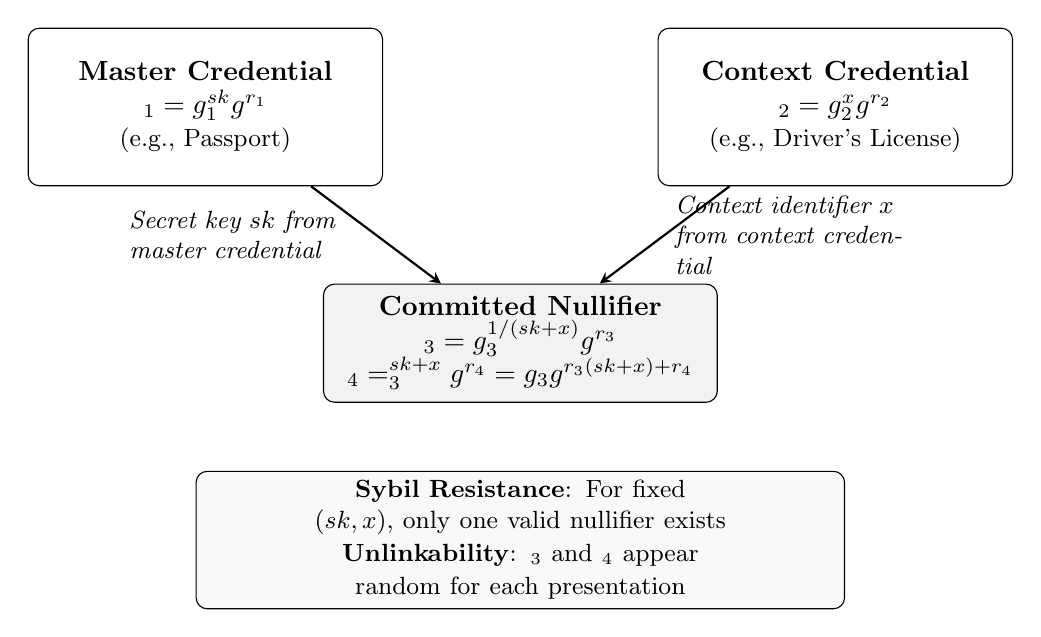
\begin{tikzpicture}[
    box/.style={rectangle, rounded corners, draw, minimum width=4.5cm, minimum height=2cm, align=center},
    nullifier/.style={rectangle, rounded corners, draw, fill=gray!10, minimum width=5cm, minimum height=1.5cm, align=center},
    arrow/.style={thick,->,>=stealth},
    label/.style={font=\small\itshape}
]

% Credential boxes
\node[box] (master) at (0,0) {
    \textbf{Master Credential}\\
    $\cm_1 = g_1^{sk} g^{r_1}$\\
    \small{(e.g., Passport)}
};

\node[box] (context) at (8,0) {
    \textbf{Context Credential}\\
    $\cm_2 = g_2^{x} g^{r_2}$\\
    \small{(e.g., Driver's License)}
};

% Nullifier box
\node[nullifier] (nullifier) at (4,-3) {
    \textbf{Committed Nullifier}\\
    $\cm_3 = g_3^{1/(sk+x)} g^{r_3}$\\
    $\cm_4 = \cm_3^{sk+x} g^{r_4} = g_3 g^{r_3(sk+x)+r_4}$
};

% Arrows and labels
\draw[arrow] (master) -- (nullifier) node[midway, left, label, text width=3cm] {Secret key $sk$ from master credential};
\draw[arrow] (context) -- (nullifier) node[midway, right, label, text width=3cm] {Context identifier $x$ from context credential};

% Sybil resistance note
\node[draw, rounded corners, fill=gray!5, text width=8cm, align=center] at (4,-5.5) {
    \small \textbf{Sybil Resistance}: For fixed $(sk,x)$, only one valid nullifier exists\\
    \small \textbf{Unlinkability}: $\cm_3$ and $\cm_4$ appear random for each presentation
};

\end{tikzpicture}
\caption{Credential Relationship Binding Nullifier connecting master and context credentials}
\label{fig:credential-nullifier-system}
\end{figure}

While our pairing-free VRF with privacy-preserving extensions addresses uniqueness and privacy, the deterministic nature of $y = g^{1/(sk+x)}$ would make presentations linkable. Our solution is to commit to the nullifier value itself, producing randomized commitments that can be verified without revealing the underlying deterministic nullifier.

\subsection{Construction}

We present two variants: a deterministic nullifier ensuring strict uniqueness, and a committed nullifier enabling unlinkable presentations while maintaining sybil resistance.

\subsubsection{Deterministic CRBN}

The deterministic CRBN directly applies our privacy-preserving VRF from Section \ref{sec:privacy-preserving-vrf}:

\begin{itemize}
    \item \textbf{Setup}: Generate group parameters and commitment bases $g_1, g_2, g \in \mathbb{G}$
    \item \textbf{MasterCredential}: Commit to master credential attributes including the secret key $sk$: $\cm_1 = g_1^{sk} g^{r_1}$
    \item \textbf{ContextCredential}: Commit to context credential attributes including the identifier $x$: $\cm_2 = g_2^{x} g^{r_2}$
    \item \textbf{NullifierEval}: Compute $y = g^{1/(sk+x)}$
    \item \textbf{NullifierProve}: Generate proof $\pi$ using Protocol~\ref{pok-committed-inverse-linear-relation}
    \item \textbf{NullifierVerify}: Verify proof $\pi$ against commitments $\cm_1, \cm_2$ and nullifier $y$
\end{itemize}

This construction ensures uniqueness but lacks unlinkability since $y$ is deterministic for each $(sk,x)$ pair.

\subsubsection{Committed CRBN}

To achieve unlinkability, we extend the construction to commit the nullifier itself:

\begin{protocol}{Proving Committed Nullifier for VRF}{committed-nullifier-vrf}\label{pok-committed-nullifier-vrf}
\textbf{Common Input:} Group generators $g_1, g_2, g_3, g \in \mathbb{G}$, commitments $\cm_1, \cm_2, \cm_3, \cm_4 \in \mathbb{G}$ \\
\textbf{Prover Input:} Witness $(sk, x, r_1, r_2, r_3, r_4)$ such that:
    \[
    \cm_1 = g_1^{sk} g^{r_1}, \quad \cm_2 = g_2^{x} g^{r_2}, \quad \cm_3 = g_3^{1/(sk + x)} g^{r_3}, \quad \cm_4 = \cm_3^{sk + x} g^{r_4} = g_3 g^{r_3 (sk + x) + r_4}
    \]
\textbf{Relation:}
\[
\mathcal{R} = \left\{ 
\begin{array}{l} 
(\cm_1, \cm_2, \cm_3, \cm_4), \\
(sk, x, r_1, r_2, r_3, r_4) 
\end{array}
\ \middle| \
\begin{array}{l}
\cm_1 = g_1^{sk} g^{r_1} \\
\cm_2 = g_2^{x} g^{r_2} \\
\cm_3 = g_3^{1/(sk + x)} g^{r_3} \\
\cm_4 = \cm_3^{sk + x} g^{r_4} = g_3 g^{r_3 (sk + x) + r_4}
\end{array} \right\}
\]
\begin{enumerate}
    \item \textbf{Commitment:} Prover samples $a_{sk}, a_x, a_{r_1}, a_{r_2}, a_{r_3}, a_{r_4} \sample \mathbb{Z}_q$ and computes:
       \[
       T_1 = g_1^{a_{sk}} g^{a_{r_1}}, \quad T_2 = g_2^{a_x} g^{a_{r_2}}, \quad T_3 = g_3^{a_{\beta}} g^{a_{r_3}}, \quad T_4 = \cm_3^{a_{sk} + a_x} g^{a_{r_4}}
       \]
       where $a_{\beta} = -a_{\beta}/(a_{sk} + a_x)$ uses a technique similar to our inverse proofs. Sends $(T_1, T_2, T_3, T_4)$ to verifier.
    
    \item \textbf{Challenge:} Verifier samples $c \sample \mathbb{Z}_q$ and sends to prover.
    
    \item \textbf{Response:} Prover computes:
       \[
       z_{sk} = a_{sk} + c \cdot sk, \quad z_x = a_x + c \cdot x, \quad z_{r_1} = a_{r_1} + c \cdot r_1, \quad z_{r_2} = a_{r_2} + c \cdot r_2
       \]
       \[
       z_{r_3} = a_{r_3} + c \cdot r_3, \quad z_{r_4} = a_{r_4} + c \cdot r_4, \quad z_{\beta} = a_{\beta} + c \cdot \frac{1}{sk + x}
       \]
       Sends $(z_{sk}, z_x, z_{r_1}, z_{r_2}, z_{r_3}, z_{r_4}, z_{\beta})$ to verifier.
    
    \item \textbf{Verification:} Verifier checks:
       \[
       T_1 \cdot \cm_1^c \stackrel{?}{=} g_1^{z_{sk}} g^{z_{r_1}}, \quad T_2 \cdot \cm_2^c \stackrel{?}{=} g_2^{z_x} g^{z_{r_2}}, \quad T_3 \cdot \cm_3^c \stackrel{?}{=} g_3^{z_{\beta}} g^{z_{r_3}}
       \]
       \[
       T_4 \cdot \cm_4^c \stackrel{?}{=} \cm_3^{z_{sk} + z_x} g^{z_{r_4}}
       \]
       
       Additionally verifies that $\cm_4 / g_3$ represents a valid randomization term (i.e., it's of the form $g^s$ for some $s \in \mathbb{Z}_q$).
\end{enumerate}
\end{protocol}

This protocol extends our previous approaches with two key innovations:
\begin{enumerate}
    \item The nullifier $g^{1/(sk+x)}$ is now embedded in commitment $\cm_3$ rather than revealed directly
    \item The auxiliary commitment $\cm_4$ enables verification that $\cm_3$ correctly commits to $g_3^{1/(sk+x)}$ by proving $\cm_3^{sk+x} = g_3 g^s$ for some randomization $s$
\end{enumerate}

The construction creates a cryptographic binding between the deterministic nullifier and the committed values, while the randomization ensures presentations remain unlinkable.

\subsection{Security Analysis}

\subsubsection{Sybil Resistance}

The CRBN provides sybil resistance through the uniqueness property: for any fixed master credential key $sk$ and context $x$, there exists only one valid nullifier value $g^{1/(sk+x)}$ that will verify correctly. Even with the committed variant, the underlying deterministic value ensures a user cannot create multiple valid credential relationships for the same context.

This uniqueness is rooted in the algebraic structure of the inverse relationship. If a user could produce two different nullifiers $y$ and $y'$ for the same $(sk,x)$ pair, both would satisfy $y^{sk+x} = g$ and $y'^{sk+x} = g$, which implies $(y/y')^{sk+x} = 1$. In a prime-order group, this is only possible if $y = y'$ or $sk+x \equiv 0 \pmod{p}$, the latter occurring with negligible probability.

\subsubsection{Privacy}

Both the deterministic and committed variants protect the privacy of credential attributes. The zero-knowledge property of our protocols ensures that nothing is revealed about $sk$ or $x$ beyond the fact that they satisfy the nullifier relationship.

In the deterministic variant, the nullifier $y = g^{1/(sk+x)}$ is pseudorandom under the $q$-DDHI assumption, appearing as a random group element to any party not knowing $sk$ and $x$. The committed variant provides even stronger privacy by hiding the nullifier value itself.

\subsubsection{Unlinkability}

The committed CRBN variant enables unlinkable presentations through randomized commitments. Each time a user presents their credential relationship, they generate fresh randomness $r_3, r_4$ for commitments $\cm_3$ and $\cm_4$. These commitments appear as new, unrelated values in each presentation, preventing linking across verifications.

The hiding property of Pedersen commitments ensures that $\cm_3$ and $\cm_4$ reveal no information about the underlying deterministic nullifier. Even a verifier who sees multiple presentations of the same credential relationship cannot determine whether they originated from the same user.






























































\subsection{Performance Evaluation}\label{sec:performance}

We implemented our constructions \cite{polgar_anonymous_2025} using the arkworks cryptography library \cite{arkworks_contributors_arkworks_2022} in Rust and evaluated performance on a MacBook Air M2 with 16GB RAM. Table~\ref{tab:performance-vrf} compares our constructions against baseline approaches, focusing on the critical operations of evaluation, proof generation, and verification.

\begin{table}[ht]
\begin{center}
\caption{Verification Time for 4 Credentials with Varying Attributes (time in ms)}
\label{tab:performance-vrf}
\begin{tabular}{l@{\hspace{1em}}r@{\hspace{2em}}r@{\hspace{5em}}r@{\hspace{2em}}r}
\toprule
\textbf{Scheme} & \multicolumn{2}{c}{\textbf{Eval + Prove (ms)}} & \multicolumn{2}{c}{\textbf{Verify (ms)}} \\
\cmidrule(lr){2-3} \cmidrule(lr){4-5}
& \textbf{ms} & \textbf{Speedup} & \textbf{ms} & \textbf{Speedup} \\
\midrule
DY$^1$ \cite{hutchison_verifiable_2005}                     & 1.27 &        & 2.2   &       \\
Our DY-PF \ref{sec-dy-pf}                                   & 0.41 & 3.1x   & 0.70  & 3.1x  \\
\midrule
DY Private \cite{tomescu2022utt}                            & 5.91 &        & 6.47  &       \\
Our DY-PF-Private \ref{pok-committed-inverse-linear-relation}                      & 1.08 & 5.5x   & 1.41  & 4.6x  \\
Our DY-PF-Private-ComOut \ref{pok-committed-nullifier-vrf}       & 2.01 & 2.9x   & 1.65  & 3.9x  \\
\bottomrule
\end{tabular}
\par\medskip
\raggedright
\footnotesize{$^1$We use optimized pairing for verification by computing all pairings in Miller Loop format before a single Final Exponentiation, reducing verify time from 2.85(ms) to 2.27(ms), a 1.26x speedup.}
\end{center}
\end{table}


Our evaluation reveals several key findings:

\begin{enumerate}
    \item \textbf{Pairing Elimination:} Our DY-PF construction achieves a 3.1× speedup over the original DY VRF by eliminating pairing operations, demonstrating the efficiency benefits of our approach.
    
    \item \textbf{Privacy Preservation Overhead:} Adding privacy preservation through commitments inevitably increases computational costs, but our DY-PF-Private design achieves a 5.5× speedup over comparable pairing-based private VRF schemes.
    
    \item \textbf{Unlinkability Trade-off:} The committed nullifier variant (DY-PF-Private-ComOut) involves additional operations for commitment handling, yet still maintains a 2.9× evaluation speedup and 3.9× verification speedup over pairing-based alternatives.
\end{enumerate}

These performance improvements have significant practical implications. The verification time of 1.65ms for our committed nullifier means that credential binding can be performed at interactive speeds on standard hardware. This enables real-time verification in applications like authentication systems, doorkey access, and mobile identity solutions.

Even with the additional privacy and unlinkability properties, our CRBN construction remains efficient enough for practical deployment in resource-constrained environments like mobile devices, where the elimination of pairing operations provides particular benefits in terms of battery usage and computational demand.

\subsection{Applications}

The CRBN enables several important applications for privacy-preserving identity systems:

\begin{enumerate}
    \item \textbf{Hierarchical Credential Systems:} Users can prove relationships between credentials from different issuers without revealing their identity or enabling tracking.
    
    \item \textbf{Private Revocation:} The nullifier can be used to implement privacy-preserving revocation mechanisms where credentials can be invalidated without compromising user anonymity.
    
    \item \textbf{One-Time Credentials:} Services can issue credentials meant for single use, with nullifiers ensuring they cannot be reused while maintaining privacy.
    
    \item \textbf{Secure Attribute Aggregation:} Organizations can verify attribute relationships across credentials (e.g., "this person's income exceeds their claimed threshold") without learning the underlying values.
\end{enumerate}

These applications demonstrate how CRBN addresses a critical gap in privacy-preserving digital identity: enabling hierarchical credential structures with binding enforceable through zero-knowledge proofs.
